\chapter{Implementation of Application Energy Monitoring}
\label{chapter:implementation}

\section{Introduction}
The logical design of the Apollo energy allocation system was presented in Chapter \ref{chapter:monitoring} and showed how, in principle, we can build a useful calculator to fairly allocate energy usage of a collection of host machines, on the basis of the individual application requests processed in a period of time (rather than just the total resource usage of application elements over a period).   Such a calculator can provide a tool for a software architect to understand the energy consumption implications of their architectural decisions and can guide them towards higher energy efficiency for the applications.

The logical design of the calculator is independent of specific technologies and does not specify the details of the implementation, simply the operations that must be performed.  Hence, as we are now to implement the calculator, the logical design acts as our specification.  Our proof of concept implementation - Apollo - can be implemented in a number of ways using a number of different technology choices and detailed design decisions.

In this chapter we explain how we went about the task of implementing our proof-of-concept calculator, the problems we set out to solve, the choices we made, some of the problems we had to solve and some of the tradeoffs that were necessary.

\section{Defining the Context}

In order to focus our attention we needed to narrow the possible design space for our problem to allow us to focus on the key decisions specific to our research rather and avoid being distracted by the generic decisions that all software projects need to make.

These basic context-setting decisions were as follows:

\begin{itemize}
	\item As mentioned in the previous chapter, We will focus on the domain of \emph{microservice-based information systems}, such as those found in large enterprises, Internet-facing systems and Internet-oriented startup companies.  We will not specifically exclude the approach being used with other architectural styles, but where a design decision is required, we will assume that the approach will be used with a microservice-based system.
	\item We will only consider our application's \emph{microservice elements and only implement monitoring of microservices that communicate via RPC calls} (typically JSON over HTTP).  These are simplifying assumptions that could be relaxed at a later point, but simplify our problem to limit the scope of our initial implementation.
	\item We will assume that the primary technology "stack" used to implement the system will be \emph{enterprise Java}, meaning software written in Java, running on the JVM, using common open source frameworks and libraries like Spring Boot, Hibernate, Dropwizard, Spring Data, Apache Commons and so on.
	\item We will assume that the primary \emph{execution platform is Linux on Intel}, as this is something of a defacto standard for running large-scale enterprise Java systems.  Where it is possible we will try to make the approach execution platform agnostic (in particular to allow for Windows, another common server execution platform in the enterprise) but again, where a decision needs to be made, we will assume a Linux on Intel host.
\end{itemize}

All of these decisions align us with mainstream industry practice and provide practical options for applying our approach to industrial systems, while narrowing our design decisions to those related to our research problem, rather than generic concerns.

We discuss each of the more specific design problems we needed to solve and the decisions we made to solve each one in the following sections of this chapter.

\section{Tracing Application Execution}

Our aim is to provide the application architect with insight into the energy consumption implications of their design decisions, and so simply measuring the energy of the infrastructure hosting the application does not provide enough information for this purpose.  The architect needs to understand the energy implications of the execution of different parts of their application, and most importantly, the energy consumption of certain types of workload.  This will allow them to understand the energy intensive parts of their application and workload and focus on improving the energy characteristics of these application elements.  Comparing the energy characteristics of different elements and workloads will also allow them to see the implications of particular design choices.

This requirement means that we need some way of tracing the execution of workload through the application to produce data equivalent to the traces and spans that we saw in Chapter \ref{chapter:monitoring}.  We considered a number of ways of achieving this.

\emph{Application specific tracing} could be provided by an application as part of its implementation and write special purpose log files or database entries to record how an application request is processed through the application's elements.  While straightforward from our perspective, this is a complex and potentially time consuming feature to add to an application and would be quite complicated to add to an existing system.  We think that this approach would be unlikely to be adopted in practice.

\emph{Application Performance Management} (APM) tools, such as AppDynamics, New Relic and Dynatrace \cite{appdynamics2018, newrelic2018, dynatrace2018} already perform application request tracing to allow them to measure and estimate application performance characteristics.  Initially using a tool like this as the basis of our approach was our preferred option.  In practice though, while attractive to practitioners who were already using the particular tool we would choose, it is a significant barrier to everyone else due to the cost and complexity of deploying these tools.  While we see our work as a potential extension of APM tools, perhaps providing them with a new dimension to their facilities, we decided against basing our approach on one of them.

\emph{Microservice tracing systems} like the open source Zipkin and Jaeger \cite{zipkin2018, jaeger2018} projects were a third alternative that we considered.  These systems are used by application developers to provide standardised trace data about the execution of their applications and provide collection and analysis infrastructure to allow the trace data to be easily used.  When we initially investigated them, they appeared to solve part of the problem of implementing application specific tracing, but still left the application developer with significant work to do.  As we investigated these open source products further we found that they are supported by or integrated into many commonly used application frameworks (for example Zipkin is already integrated into libraries for about 10 languages, including Java, Python, C\# and JavaScript, and just considering Java, it is integrated into more than 15 well known application frameworks including Spring Boot, Dropwizard, Google RPC, Apache HTTP Client and Jersey).  If using a pre-integrated framework, using these tracing systems is very straightforward from an application developer's perspective and normally simply involves starting the data server to receive the trace data and setting some configuration parameters in the framework configuration.

After some experimentation we found that the Zipkin tracing system worked very well for a set of Java microservices and its database was easy to query to extract the trace information we needed.  We concluded that the reliability, easy availability, low implementation overhead, ease of use and large number of existing integrations with widely used application frameworks made Zipkin a good choice for our work.

\section{Estimating Resource Usage of Application Workload}
\label{section:resusageofappworkload}

Once we can reliably trace execution of application requests through the application elements involved in processing them, we can move to considering how to estimate the resource usage of those application elements in order to work out the resource consumption of the requests processed by the application.  The key requirement here is to be able to collect reliable samples of the resource usage of the application elements on a very frequent and predictable basis (e.g. every couple of seconds).  Ideally the samples will be in terms of cumulative usage rather than usage at that point in time, as these are much easier to use for our purposes.

The only practical source of application resource usage statistics is the application execution platform.  There are a number of sources of statistics that we could use, each with slightly different characteristics.

The simplest option is to use \emph{native operating system tools} such as \texttt{sar} and \texttt{pidstat} on Linux and \texttt{procmon} and \texttt{perfmon} on Windows.  In principle these tools can collect resource usage statistics for application processes on the machine.  However in practice, our industrial experience and recent investigation for this work, suggests that they are really intended for collecting host-level statistics or for interactive investigation of a performance problem on a machine, by a skilled administrator.  They do not provide an easy way to get a reliable stream of samples of cumulative usage over time written into an accessible form.

An alternative is to bypass the tools and access the \emph{operating system performance counters} directly.  Like most modern operating systems, Windows and Linux both implement a set of performance counters in their kernels, which are used for monitoring performance and throughput of workload executed by the machine.  These counters are used by the operating system tools to provide the data they need to operate and so by accessing the counters directly, we can avoid any limitations in the tools and still achieve consistent results.  Linux provides access to its performance counters via the very convenient \texttt{{/proc}} file system, which exposes all of the kernel's counters for global and process-specific metrics, via a pseudo file system interface (which can be read using standard text processing tools or through the standard file system API).  Windows provides access to its performance counters via the \texttt{perfmon} tool or through an API which is accessible via PowerShell (the modern Windows scripting language) or a conventional programming language.  In principle we can build any collection tool we want using these interfaces or we can use metrics collection servers such as \texttt{telegraf} or \texttt{collectd} \cite{telegraf2018, collectd2018} to read them automatically and store them in a suitable database for us.  During initial research, this approach was our preferred option, however in practice we found it quite difficult to get a usable set of statistics for our application.  The main problem we faced was that the collector does not know which workload on the machine belongs to a particular application.  Therefore we had to collect everything at operating system process level, which potentially generates huge amounts of unnecessary data.  We also found that the business of building a reliable collector was more difficult than initially assumed and that linking the trace data to the dataset we could collect easily from operating system counters was quite difficult to do reliably.  These difficulties were not insurmountable, but led us to consider whether there were other options we could consider.

The third option we investigated was to use \emph{Docker} \cite{docker2018} as a packaging technology for the application elements and to allow us to collect resource usage statistics.  Docker is an operating system virtualisation technology which uses operating system mechanisms (such as "cgroups" and "kernel namespaces" on Linux) to isolate processes from each other, providing the illusion that each is running on a separate machine.  Docker also provides a packaging convention that allows software to be packaged into reusable packages called "images" which are combined at runtime to form runtime environment known as a "container".  Docker also provides a set of management APIs and tools to allow containers to be interrogated, managed and controlled.  Docker is rapidly becoming a de-facto standard in the industry to package, deploy and manage microservices both on general host computers (where Docker becomes an execution environment on top of the operating system) and more abstract, container based platforms like Kubernetes \cite{kubernetes2018} where Docker forms part of a sophisticated platform providing demanding quality properties like scalability and resilience, across a cluster of host computers.

Our interest in Docker lies in its ability to provide a low-overhead, isolated environment for running application elements (in our case, microservices specifically).  If we can assume that all of the microservices within our system are packaged and then run as Docker containers then it provides us with the ability to extract accurage resource utilisation statistics for the microservice running in the container.  Another benefit of using Docker is that each container has its own network (IP) address which can be found via the runtime metadata available via Docker's management API.  This greatly simplifies the process of relating the resource usage data to the request traces from Zipkin as the network address is a shared piece of information between the two.

We believe that requiring application elements (the microservices) to be packaged and run as Docker containers is realistic and reasonable, given its wide and growing adoption in industry, particulary for microservice-based systems.  Therefore this combination of factors resulted in us deciding to use Docker as the basis for collecting application resource utilisation statistics.

A useful side effect of packaging the application as a set of microservices in containers is that it makes the utilisation of the trace data simpler.  The trace data identifies the application elements by network address (typically IP address and port number).  Each container in a Docker deployment (strictly a Docker network) has its own set of one or more IP addresses.  Therefore, by having each application element in a separate container, we can rely on them listening on different IP addresses and for the container to IP address mapping being available from the Docker meta data.  Hence this approach to application packaging and deployment makes the mapping of trace data to application elements straightforward. 

The second part of collecting utilisation statistics is how they are extracted and stored from the execution platform.  In our case, our experimentation with Docker quickly revealed that a number of open source projects, including \emph{cAdvisor} \cite{cadvisor2018} and \emph{Telegaf} \cite{telegraf2018}, provide close integration with Docker and can extract and store the utilisation statistics data in different database systems.

After some experimentation we chose to use Docker with Telegraf, storing utilisation statistics in the \emph{InfluxDB} \cite{influxdb2018} open source time-series database to provide us with reliable application element resource utilisation statistics gathering.

\section{Estimating Resource Usage of the Host Platform}

Estimating resource usage of the underlying host platform is simpler than gathering the same information for the application elements, as host-level statistics gathering is a mature and widely used technology, provided by all major operating system platforms.

In our case we need to achieve reliable resource utilisation sampling of the host platform - the underlying Linux operating system - and have them stored in a database that allows us to extract them through a query interface to support the calculation process.  Ideally if the statistics are in a similar form to the statistics for the application level resource utilisation (e.g. the same timestamp convention and data types used), then this is likely to make the implementation of the calculator easier.

Our earlier investigation of the \emph{Telegraf} data collection server to extract and store application-level utilisation statistics revealed that it can be configured to extract and store host-level utilisation statistics too, and that this facility is provided as part of the standard distribution of the (open source) product.  When we tested the host resource utilisation statistics feature of Telegraf we found that it was straightforward to use and reliably stored accurate statistics in the same database as the application-level statistics.  The host-level statistics used the same basic conventions as the application-level statistics (e.g. they were both cumulative utilisation statistics using the same timestamp conventions).

Therefore we were able to solve the host-level resource utilisation statistics gathering problem by simply extending the configuration of the Telegraf server and the extension of the data set it stored to include host-level statistics.

\section{Estimating Energy Usage of the Host Platform}

As explained when we discussed the motivation for this work in Chapter \ref{chapter:introduction} the field of energy estimation is relatively young and reliable approaches for energy estimation of individual devices and applications are only just emerging.  Our work does not intend to address the problem of estimating energy consumption for a single host computer, but rather requires a reliable energy consumption metric to be available.

As explained in Chapter \ref{chapter:monitoring} there are two main approaches available to us that can provide energy usage of our underlying host platform, physical energy consumption metrics made available via a DCIM platform and model-based energy consumption estimation using machine utilisation levels and published benchmark results.

In many industrial situations a DCIM platform will be available and energy consumption metrics for all or a significant subset of host machines will be available through it.  However in our research environment we did not have access to such a platform and in many industrial situations this will be the case too.  While the state-of-the-art in organisation design is to integrate development and operations groups, they are frequently still separate and so even when a DCIM platform is available, software architects may well not be able to access it easily.

Therefore we decided to use a model-based approach to estimate the energy consumption of the host, but to ensure that it was easily replaceable with alternative models or with queries to a DCIM platform if one was available.

The approach used to estimate the energy usage of a host was explained in section \ref{subsection:calculation-specification} and relies upon published power consumption benchmark results associated with the SPECpower\_ssj 2008 benchmarks \cite{lange2009-specpower}.  An example data set for power consumption for a specific model of server host is shown in \ref{table:powervalues}.

\begin{table}
\centering
%  (Intel Xeon E5-2699 v4 2.20 GHz)
\caption{SPECPower 2008 Benchmark Results for \\Dell R730 Poweredge}
\label{table:powervalues}
\footnotesize
\begin{tabular}{|c|c|c|}
\hline
Machine Load & Power Consumption (W) & W / \% \\
\hline
\hline
Active Idle  &  44.6 & -    \\
10\%         &  84.8 & 8.48 \\
20\%         & 102.0 & 5.10 \\
30\%         & 120.0 & 4.00 \\
40\%         & 136.0 & 3.40 \\
50\%         & 150.0 & 3.33 \\
60\%         & 163.0 & 2.64 \\
70\%         & 181.0 & 2.58 \\
80\%         & 205.0 & 2.56 \\
90\%         & 238.0 & 2.64 \\
100\%        & 272.0 & 2.72 \\
\hline
\end{tabular}
\end{table}

We use this style of benchmark data combined with the machine type executing our application workload and the utilisation level metrics of the server executing the load to estimate host server energy consumption at a particular point in time, as explained in section \ref{subsection:calculation-specification}.

The third column in the table is a derived value we have added to show the power consumption per percentage point of server utilisation at each level of utilisation.  This clearly illustrates the need to keep servers busy from an energy efficiency perspective as it can be seen clearly that 1\% utilisation when the machine is quiet is three times more expensive in energy consumption terms than 1\% utilisation when the machine is busy.  We investigate this observation further in Chapter \ref{chapter:validation} when we describe how we validated the implementation of Apollo.

\section{Implementing the Calculator}

\subsection{Design of the Calculator}

The design of the Apollo calculator is shown in the simple block diagram in Figure 3. The system element filled with the fine dotted pattern represents the architectural elements of the application (i.e. an application microservice), the system elements filled with the fine cross-hatching are data elements, while the Apollo Energy Estimator is filled with the light solid fill.  The unshaded elements are the third party technologies which are reused unchanged as part of the implementation.

\begin{figure}
\centering
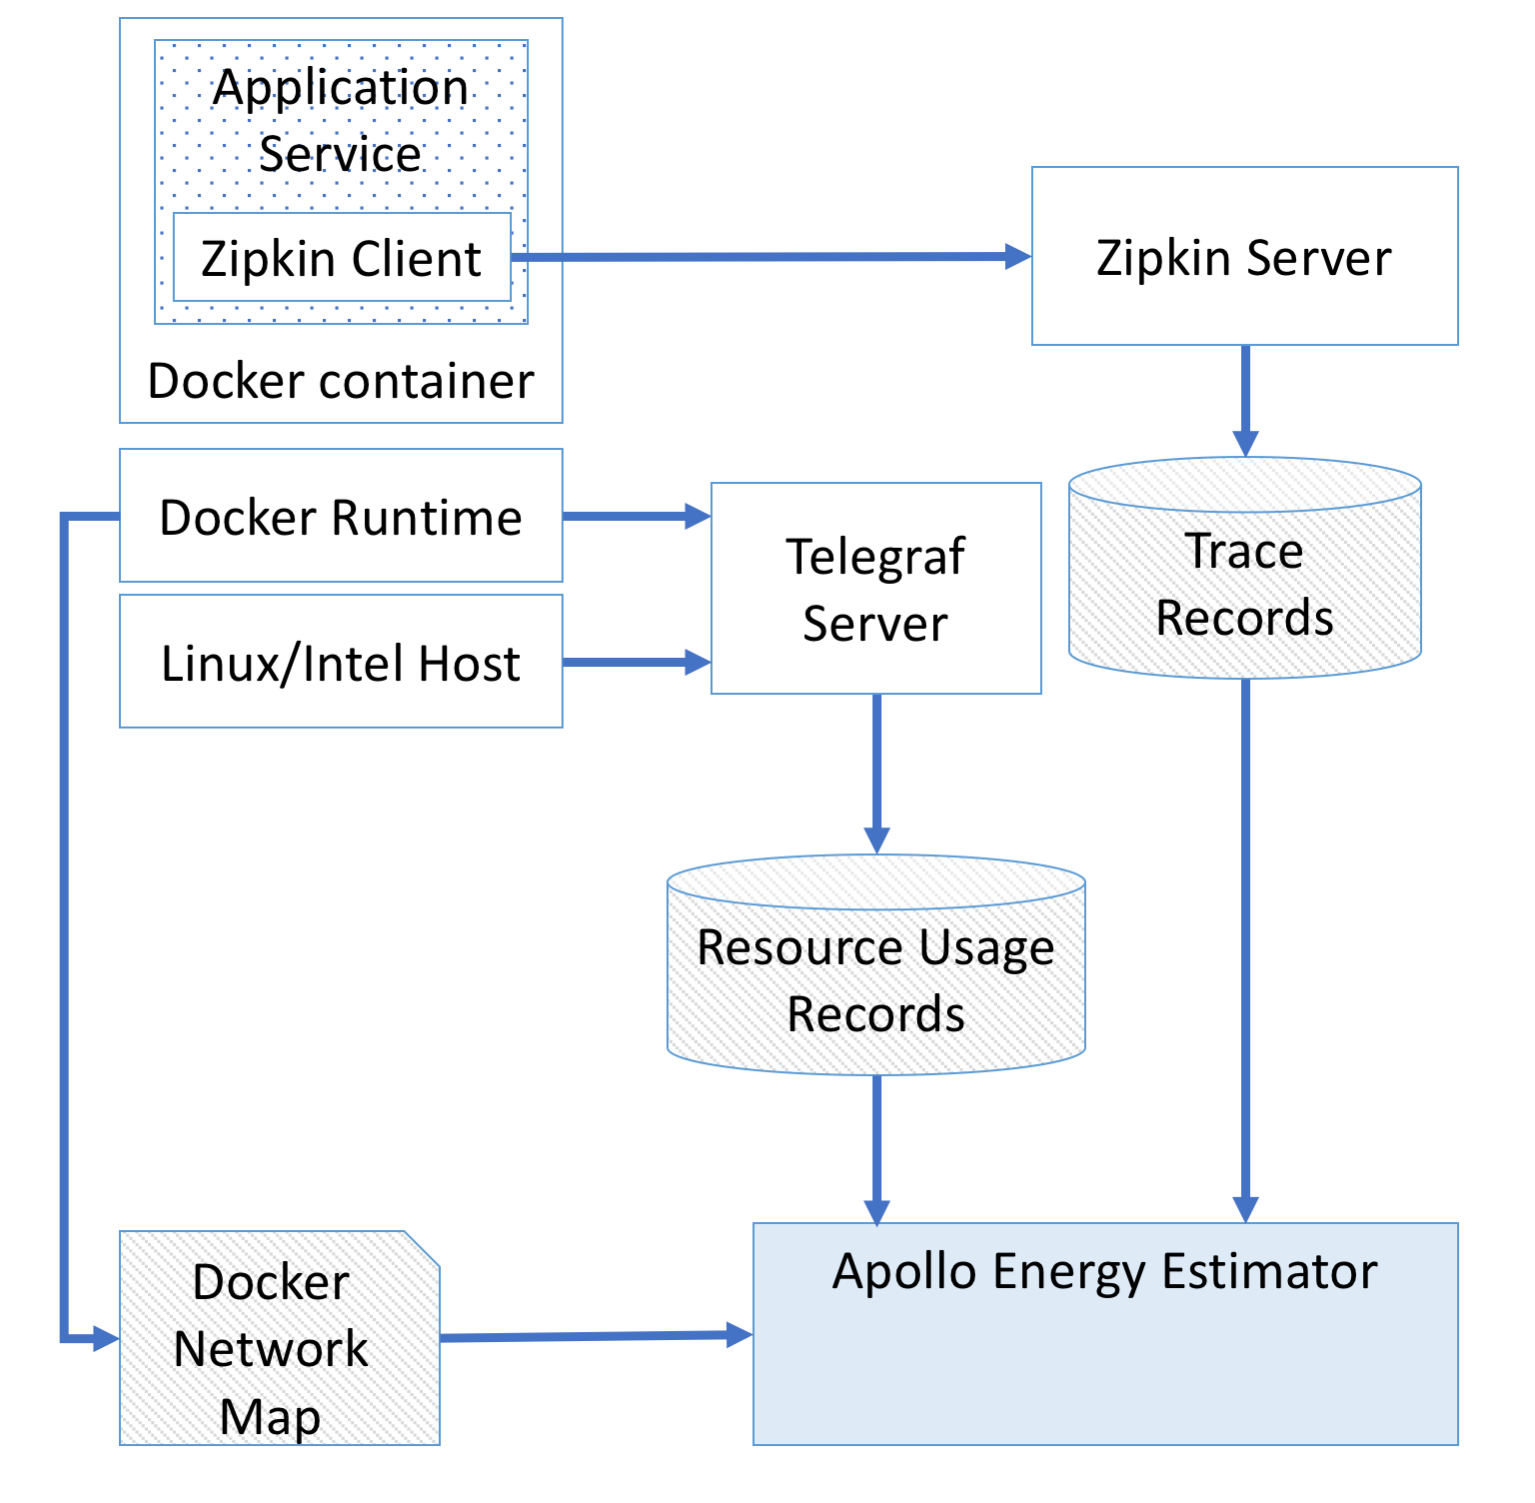
\includegraphics[width=0.5\textwidth]{Figures/implementation-design}
\caption{Design of the Apollo Energy Calculator}
\label{figure:implementation}
\end{figure}

The design elements of the calculator and their responsibilities are summarised in Table \ref{table:designelements}

\begin{table}
\centering
\caption{Apollo Energy Calculator Design Elements}
\label{table:designelements}
\footnotesize
\begin{tabular}{|l|p{10cm}|}
\hline
\textbf{Design Element} & \textbf{Responsibilities}  \\
\hline
\hline
Application Service & This element represents the regular microservices that comprise the application under investigation.  The implementation of these services are under the control of the development team and they have the responsibility to generate Zipkin trace records (via the Zipkin Client library) to record their activity (although this will usually be achieved automatically through use of an application framework like Spring Boot). \\
\hline
Zipkin Client & A trace of the invocations to and between application elements is required and as explained above, the Zipkin tracing system is used to achieve this.  The Ziplin Client is a client programming library used by Application Services to generate trace records and forward them to the Zipkin Server for storage.  The application code may invoke this library directly or it may be invoked automatically by an application framework like Spring Boot or Drop Wizard. \\
\hline
Zipkin Server & The Zipkin server receives and stores the trace records from the Application Services.  One Zipkin Server is used for all of the Application Services in a monitoring context. \\
\hline
Trace Records & The Zipkin Server persists the trace records in a well defined schema in a database.  In our case we used MySQL as the database for the trace records. \\
\hline
Docker Container    & All application elements need to run within Docker containers.  This allows metadata about the elements to be retrieved and resource usage statistics to be gathered.  This container contains the Application Service (each service is packaged in a separate container to allow it to be monitored separately).\\
\hline
Docker Runtime     & The Docker Runtime is part of the Docker system software package and provides the control and monitoring of the Docker containers in the application and provides runtime statistics for the containers, which in our situation are streamed to the Telegraf Server for storage. \\
\hline
Linux/Intel Host   & The application runs within Docker on the underlying host machine(s) and we have chosen to use an Intel host running the Linux operating system, due to the maturity of both Java and Docker on this platform. \\
\hline
Telegraf Server & The Docker platform produces a stream of resource usage statistics for the containers that it is executing.  The Telegraf open source metrics collection agent collects these metrics and stores them in a timeseries database for easy retrieval. \\
\hline
Resource Usage Records & The Telegraf Server generates a stream of resource utilisation statistics by constantly querying the Docker Runtime and the Linux Host.  These statistics records are persisted to a database for later use.  The datastore used for the Resource Usage Records is InfluxDB, an open source timeseries database. \\
\hline
Docker Network Map & The Zipkin traces and the resource usage records identify the runtime elements of the system in different ways; the Zipkin traces are collected at the network level and so identify elements by IP address and port number, while the Docker resource usage statistics are identified by Docker container ID.  Hence metadata is needed to link the two together and this is the purpose of the Docker Network Map which is metadata available from the Docker Runtime (through the \texttt{docker network inspect} command) which allows us to find the IP address(es) in use by each container during the execution of the application. \\
\hline
Apollo Energy Estimator & The Apollo module collects data and implements the energy allocation algorithm described in Chapter \ref{chapter:monitoring}.  This module is the primary software that we have implemented as part of this research (along with an example application we use for validation, which we describe in Chapter \ref{chapter:validation}). \\
\hline
\end{tabular}
\end{table}

Most of the system described here is open source software (Docker, Telegraf, Zipkin, InfluxDB, MySQL and Linux) and so the only significant piece of custom software that had to be developed for this investigation was the Apollo Energy Estimator module.  The other software development effort was configuration and scripting to combine the different pieces of software into a single system.  We describe the software design of the Estimator module in the next section.

\subsection{Data Design}
\label{subsection:data-design}

In the earlier subsections, we explained how we would solve each of the data gathering problems in order to create the data sets that the energy estimator requires in order to perform its calculations.  We now need to define how that data is used by the calculation code.

The data model for the data from the different sources is shown using the UML class diagram in Figure \ref{figure:data} and the data elements are described in Table \ref{table:dataelements}.

\begin{figure}
\centering
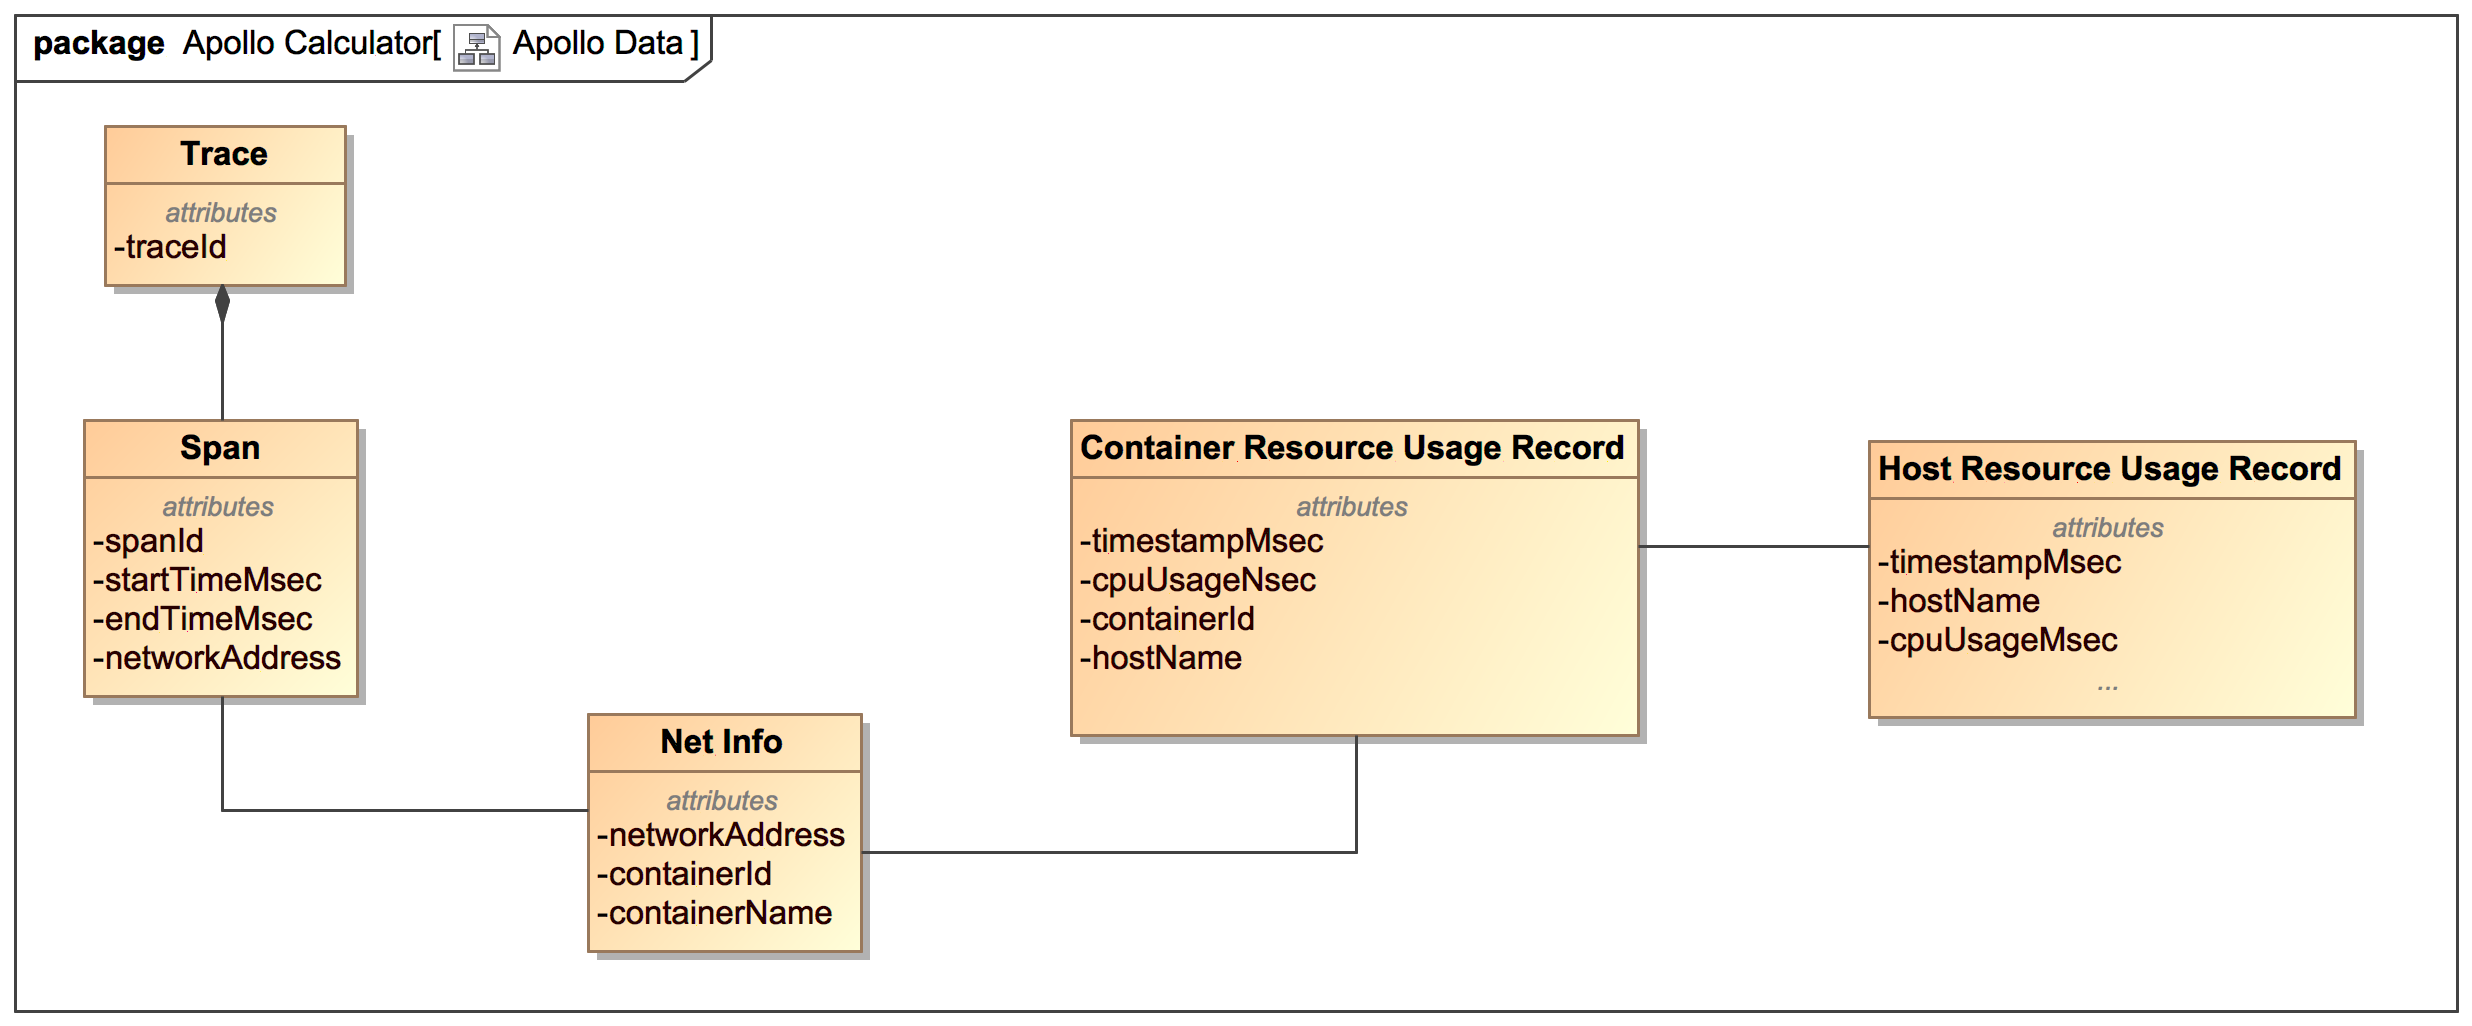
\includegraphics[width=1.0\textwidth]{Figures/implementation-data}
\caption{Data Structure for Apollo Energy Estimator}
\label{figure:data}
\end{figure}

\begin{table}
\centering
\caption{Apollo Energy Calculator Data Elements}
\label{table:dataelements}
\footnotesize
\begin{tabular}{|p{4cm}|p{9.5cm}|}
\hline
\textbf{Data Element} & \textbf{Description}  \\
\hline
\hline
Trace & The \textit{Trace} is just a simple container for a set of \textit{Spans}.  While the Zipkin data item does contain more information, from our perspective, we are only interested in it having a unique ID.  This is sourced from the Zipkin data set.\\
\hline
Span & Contains the information recording a specific invocation of an application element.  One \textit{Span} is written for each application element invoked as part of a trace.  Identifies the application element by \textit{networkAddress} (an IP address in our case) and records the start and end time of the invocation in milliseconds.  Composed into exactly one \textit{Trace} and so contains its ID to record the relationship.  This is sourced from the Zipkin data set. \\
\hline
Net Info & Provides a mapping between network addresses, (Docker) container IDs and container names.  Any network address maps to exactly one container ID and one container name.  This is sourced from the Docker Network Map data set. \\
\hline
Container Resource Usage Record & Records the resource usage of a specific container at a point in time.  Contains the sample time as a millisecond timestamp, the cumulative CPU usage in nano-seconds measured at that point, the ID of the container being measured and the hostname of the computer it was executing on. This is sourced from the Docker resource utilisation statistics collected by Telegraf (and stored in InfluxDB).\\
\hline
Host Resource Usage Record & Records the resource usage of a host computer at a point in time.  Contains the sample time as a millisecond timestamp, the cumulative CPU usage in milliseconds measured at that point and the hostname of the machine.  This is sourced from the operating system resource utilisation statistics collected by Telegraf (and stored in InfluxDB). \\
\hline
\end{tabular}
\end{table}

The basic data access path required is to start with the \emph{Trace} and iterate over the \emph{Spans} that it contains.  For each span, use the \emph{networkAddress} to identify the service endpoint and use the \emph{Net Info} data to map this to the \emph{containerId} that executed the span's request.  This allows the resource usage records for the container to be identified using the container ID and the start and end time of the trace.  Then, to establish the resource utilisation of the host during the same period, the \emph{hostName} attribute of the \emph{Container Resource Usage Record} and the start and end times can be used to identify the correct \emph{Host Resource Usage Records} to use.

Therefore, as can be seen, this data stucture allows us to navigate through the data sets to find container and host resource utilisation data for each of the spans in a trace.

There is one remaining problem however, which is the fact that the spans are periods of time, but the usage records are samples at a point in time.  We need to solve this problem to use the data correctly.

In our specification, in Section \ref{subsection:calculation-specification} we specified the use of interpolation to estimate the CPU usage between the two points surrounding the start and end of the trace and then calculating the difference between the two cumulative CPU usage values for each container involved in handling the request.  

This approach works well when the trace period crosses a number of sample intervals and we confirmed this early in the process using practial testing.  However, when using the technology it is important to be aware that when the trace period is very short compared to the sample interval, and so all of the execution occurs within one sample interval, the interpolation estimation is too coarse to produce accurate results for the CPU usage.  This is simply a limitation of using sample intervals for resource usage estimation and is a familiar problem in performance monitoring and analysis work.

As we investigated the technologies that could provide resource utilisation metrics, we discovered that sample intervals for real resource utilisation statistics, such as those provided by operating systems or Docker, are actually very long when compared to request durations.  A typical sample interval for Docker is 10 seconds and an operating system might be 1 minute, whereas the duration of a simple request may only be tens to hundreds of milliseconds.  Sample intervals can be reduced in duration (at the cost of monitoring overhead and data volume) but realistically they can only be reduced to 5 - 10 seconds, not the durations that match request durations.

The solution to this is simply to run the workload multiple times, so that the measurement is made over a number of sample intervals, at which point the error from the interpolation is insignificant in the overall estimate.  With standard Docker and Linux monitoring through Telegraf we found that 5 more sample intervals was sufficient (so 50 seconds with a sample interval of 10 seconds).  While real application traces would not be this long, it is a common constraint for performance monitoring work.  Given that we are running dedicated microservice instances for energy estimation and assuming synthetic testing workload run in the production environment (as explained in Section \ref{subsection:calculation-specification}) then this constraint is unlikely to be a problem in practice.


\subsection{Software Design and Implementation}

The Apollo estimator does two primary things, it gathers data from the resource utilisation statistics, the trace records and the Docker network meta data and it uses the information to perform the energy allocation processing required to establish the energy characteristics of each of the inbound requests to the application, described in the trace records. 

The implementation of the module is described by the UML class diagram in Figure \ref{figure:classes} and the class descriptions in Table \ref{table:classes}.

\begin{figure}
\centering
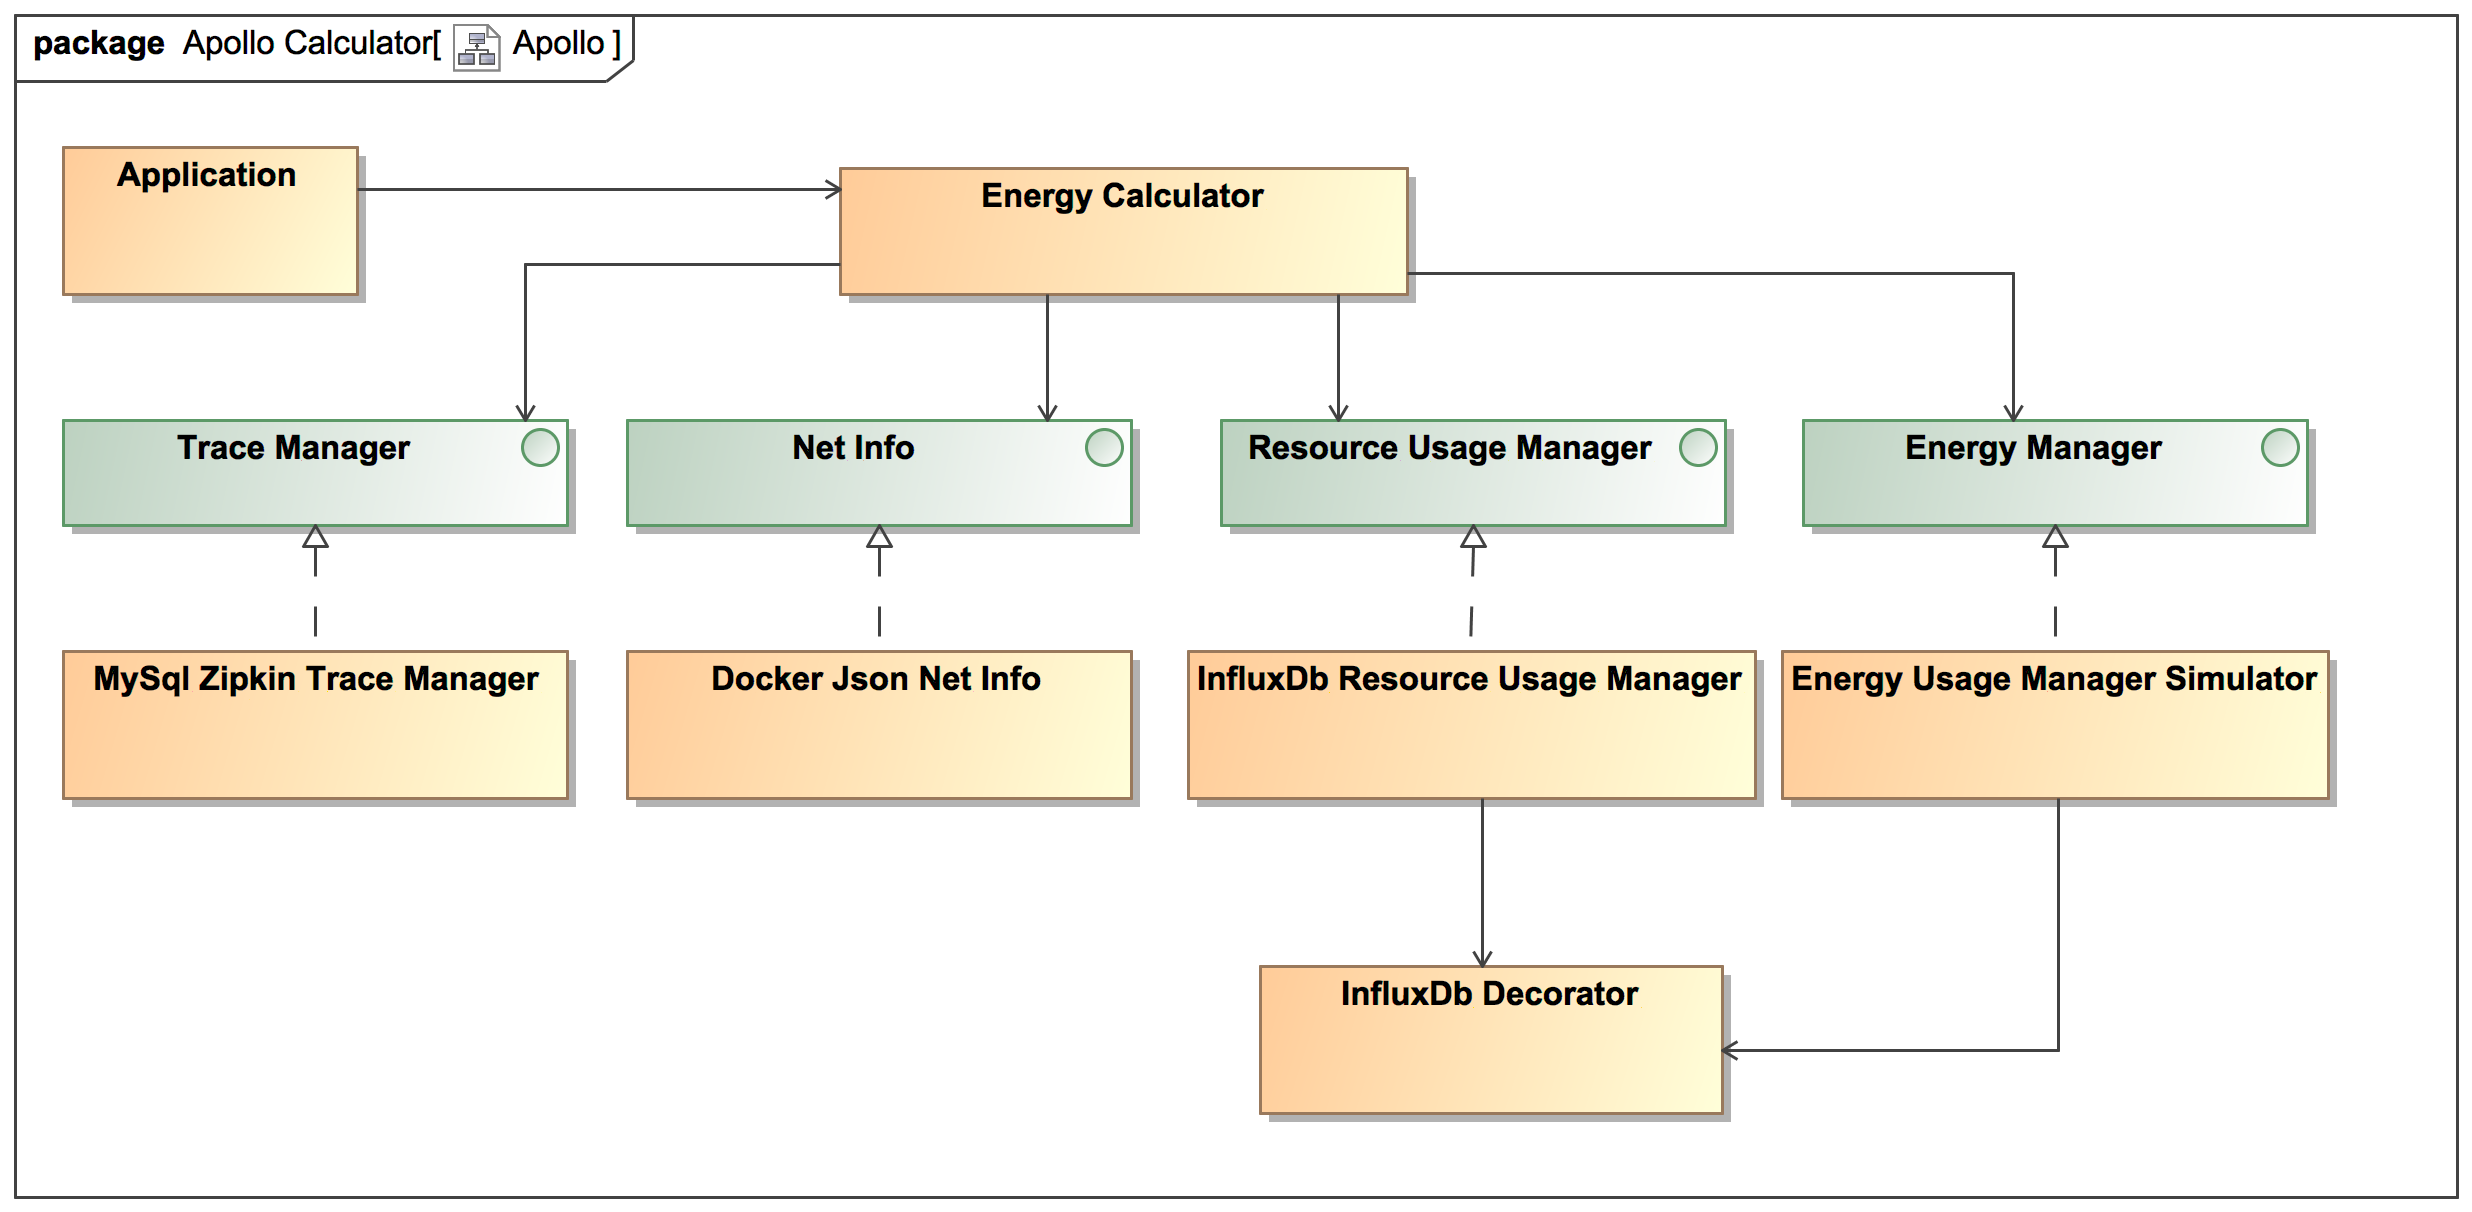
\includegraphics[width=1.0\textwidth]{Figures/implementation-classes}
\caption{Implementation of the Apollo Energy Estimator Module}
\label{figure:classes}
\end{figure}

\begin{table}
\centering
\caption{Apollo Energy Estimator Module Structure}
\label{table:classes}
\footnotesize
\begin{tabular}{|p{4cm}|p{9cm}|}
\hline
\textbf{Design Element} & \textbf{Description} \\
\hline
\hline
Application & This is a small "bootstrap" class with the responsibility of loading configuration settings, creating the other elements and providing an entry point for the runtime system. \\
\hline
Energy Calculator & Provides the main processing loop to retrieve traces from the \texttt{Trace Manager}, retrieve the corresponding data for each trace from the other elements and then perform the required calculation. \\
\hline
Trace Manager & An interface defining a simple API to retrieve trace records. \\
\hline
MySql Zipkin Trace \newline Manager & An implementation of the \texttt{Trace Manager} interface that accesses the Zipkin Server's MySQL database to retrieve the trace records held within it. \\
\hline
Net Info & An interface defining a simple API to allow container IDs to be mapped to network addresses and vice versa and container names to be mapped to container IDs and vice versa. \\
\hline
Docker Json Net Info & An implementation of \texttt{Net Info} to provide the container name, ID and network address mappings from the JSON file produced by the Docker \texttt{docker network inspect} command. \\
\hline
Resource Usage Manager & An interface describing the API to retrieve resource usage information during a period of time for a Docker container, for a host machine or for a host machine where a specific container ran. \\
\hline
InfluxDb Resource Usage \newline Manager & An implementation of \texttt{Resource Usage Manager} that retrieves the information from an InfluxDB that has been populated by the \texttt{Telegraf} metrics capture server. \\
\hline
Energy Usage Manager & An interface defining the API that provides the ability to retrieve energy usage information for a host machine by name for a period of time, or a host machine that a particular container ran on during a period of time. \\
\hline
Energy Usage Manager \newline Simulator & An implementation of the \texttt{Energy Usage Manager} interface that uses a simulation based approach to provide realistic energy consumption information. \\
\hline
InfluxDb Decorator & A key utility class that implements the Decorator pattern and adds functions and ease-of-use features to the standard \texttt{InfluxDB} Java client class for InfluxDB.  This allows all of the schema navigation and query language specifics to be isolated and hidden in this class. \\
\hline
\end{tabular} 
\end{table}

The interaction between the classes is fairly straightforward.  Some of the code within the classes (such as that needed to retrieve and transform data into a suitable set of types to make the calculations straightforward) is intricate, but none of it is particularly complex algorithmically.

The flow of control between the modules is quite straightforward and follows the layout of the classes on the diagram; it can be summarised as:

\begin{itemize}
	\item The Application is invoked, it loads its configuration settings from a configuration file, creates instances of the other objects, "wires" them together and invokes the Energy Calculator.
	\item The Energy Calculator calls the Trace Manager to retrieve all of the traces in the current data set and for each one:
	\begin{itemize}
		\item calls the Net Info class to find the set of containers that were invoked (by mapping the network address from a span record to the container ID);
		\item calls the Resource Usage Manager to retrieve the resource usage data for the containers;
		\item calls the Resource Usage Manager to retrieve the resource usage data for the hosts the containers were executed on;
		\item calls the Energy Usage Manager to retrieve the energy usage of the hosts during the time period of the trace; and
		\item calculates an estimate of the energy allocation of the trace, based on the estimates of the energy allocation of each container that it can calculate using this information.
	\end{itemize}
	\item The Application then reports the energy allocation of each trace using the information returned from the Energy Calculator. 
\end{itemize}

We discuss how we implemented the algorithm in more detail in section \ref{subsection:algorithm}.

The Energy Estimator module was implemented using mainstream, modern, development technology from the Java Virtual Machine (JVM) ecosystem.  The primary implementation language was Kotlin \cite{jemerov2017-kotlin}, which was chosen for its ease of adoption, its strong support for interoperability with existing Java libraries and its functional language features.  Much of the core calculation involved sets, lists and maps and functional programming features made this code significantly shorter than would have been the case using a traditional imperative style in Java. 

The code was developed in a largely test driven style with unit and integration tests being developed with the main code and an automated build, implemented using Gradle, running all of the tests before creating the delivered binary package.

A significant amount of open source software was used in the implementation, which dramatically reduced the amount of software that needed to be written.  The key external libraries used in the main code were \emph{Spring JDBC} to access the MySQL database, \emph{InfluxDB-Java} to access the InfluxDB database, \emph{Klaxon} to provide JSON binding and \emph{Konfig} to handle configuration settings. 

The Energy Estimator module is about 1500 lines of code with about 1250 lines of associated test code.  Kotlin's brevity and functional programming features contibuted significantly to keeping the number of lines of code needed low.  There are also about 1500 lines of associated script and resource definition code for automation of environment setup and execution.

\subsection{The Calculation Algorithm}
\label{subsection:algorithm}

In Section \ref{subsection:calculation-specification} we presented the specification of how to perform the energy allocation process as a series of equations.  Having designed a practical approach to collecting and estimating the input data for this process, we now had to implement an algorithm that would perform the calculation processed as specified.  In this section, we highlight the significant steps that we took in this process.

The first step was to implement \emph{Trace} and \emph{Span} abstract data types, along with a set of types to store resource usage measurements.  These class were all implemented using Kotlin's data class construct.  The key decisions were to use a string representation for network addresses (to allow different sorts of network address without code change) and for all times and durations to be stored as millisecond precision timestamps since the Unix "epoch".

The next stage in implementation was to implement the \emph{Trace Manager}, and \emph{Resource Usage Manager} interfaces and their implementing classes.  These classes provide access to the MySQL database containing the Zipkin trace records and the InfluxDB database containing the Docker and host resource usage statistics records respectively.  Both of these classes are relatively sophisticated in the sense that they encapsulate the complexity of navigating the database models and mapping the data returned by the databases in order to provide a simple interface to calling code, using the abstract datatypes implemented in the previous step.  The MySQL implementation of the Trace Manager relies heavily on Spring Data and the MySQL Java Connector library classes to simplify query execution and result set handling.  The InfluxDB implentation of the Resource Usage Manager uses the standard InfluxDB Java client to access the database.

Once we had reliable, tested, access to the databases, the \emph{Net Info} interface and its Docker specific implementation was implemented.  It reads a JSON file generated by the \texttt{docker network inspect} command and extracts a network address to container ID to host name mapping from it.  It use the Klaxon open source library to provide idomatic access to JSON data from Kotlin, which made the implementation fairly straightforward.

It was now possible to embark on the initial implementation of the \emph{Energy Calculator} which was implemented as two classes, the main Energy Calculator class that retrieves the traces from the Trace Manager and iterates over them, and a helper \emph{Trace Calculator} class that performs the energy allocation calculation for one trace.

The Trace Calculator makes extensive use of Kotlin's functional programming features and related data types (maps, sets and lists).  The data is extracted from an SQL database, a JSON file and a No-SQL timeseries database.  Therefore it can't simply be accessed via a single database query, which might have been an option if it had all been in a single relational database.  Instead, this class reads subsets of the data of interest from the data stores and converts them to maps and lists structured to make the required computation straightforward (for example the Net Info data is transformed from a JSON struture to a set of maps from networkAddress to containerId, containerId to networkAddress and containerId to containerName).  This then allows extensive use of functional programming constructs like \texttt{map}, \texttt{reduce} and \texttt{fold}, which resulted in compact code that reflected the essentials of the algorithm well.

At this point, the software could run reliably against a data set and calculate CPU usage and the percentage of total host CPU that the trace represented during its execution.

The next stage was to implement the \emph{Energy Usage Manager} interface and its concrete implementation the \emph{Energy Usage Manager Simulator} class, which provides estimates of energy consumption for a specified machine during a specified period.  This implementation uses a model based approach, utilising SPEC Power benchmark energy values for the machine type of the host.  The class queries InfluxDB to find the host CPU utilisation during the specified time period for the specified host and then uses a lookup table to find an estimate of the power consumption for the host type of the machine at the average level of utilisation during the period.

This completed the implementation of the calculation module and its automated tests, allowing us to move on to the validation stage and use it to perform energy allocation calculations for real test cases for a sample application, which we describe in Chapter \ref{chapter:validation}.

\section{Limitations of the Apollo Energy Estimator}

Our implementation of the Energy Estimator is a practical proof of concept version which we have used to run extensive tests to validate its implementation and the general approach for energy usage allocation for an application's request processing.  There are however a number of known limitations in the current implementation, some of which are fundamental to our approach and some of which are the result of simplifying decisions to make the proof-of-concept implementation tractable, and which could easily be addressed through further work.

Firstly the estimator does not take \emph{infrastructure energy consumption} into account as part of its calculation.  A data centre's energy efficiency is normally measured through its \emph{Power Usage Effectiveness - PUE} ratio \cite{iso30134-pue}, which measures the ratio between the energy used for computing equipment and the overall energy consumption of the data centre.  The difference between the two is the data centre's infrastructure energy consumption due to items like lighting and cooling.  For simplicity of initial implementation, the estimator does not take PUE into account and so ignores the infrastructure energy overhead.  This would be reasonably straightforward to add, given a source of data to define the PUE ratio at different times of day for the data centres where the execution hosts are resident.

As we noted at the start of this chapter, we have made a simplifying implementation decision to only monitor the \emph{energy consumption of our application microservices that communicate using RPCs} (usually JSON over HTTP, although this is not in fact a limitation of the implementation - using Zipkin we can trace over other transports such as gRPC too).  This assumption reduced the number of special cases we need to consider in the proof-of-concept implementation and could be relaxed at a later date.  Zipkin is capable of tracing service invocations over other transports (like messaging) and we could extend the approach to allocate energy correctly to other elements of the architecture (like database servers dedicated to our microservices), by extending the sophistication of our implementation.  What we can't easily estimate is energy consumed by "side effects" of the execution of our system, such as the energy consumed by another system as the result of us sending it a message.  If the appoach is implemented in all of the systems then all of the energy will be allocated somewhere, but in reality this is unlikely ever to be the case, hence we exclude the energy impact of external side effects.

Next, the approach we use has a \emph{reliance on dedicated microservices} ("runtime elements") for testing purposes.  This is because we cannot separate the resource usage by a microservice for our traced requests from the overall resource usage of the microservice if it is used for other work during the period of the trace.  This is a reasonably fundamental limitation of using resource utilisation metrics at the microservice level.  On some operating systems (such as Linux) it is possible to obtain CPU utilisation metrics at thread level, which would allow more flexibility in this regard.  However it would need us to make quite a sophisticated extension to a tracing library like Zipkin or Jaeger to map requests to execution threads as well as network addresses, and so we did not attempt this during the proof-of-concept implementation, but will consider it as a possible future direction for the work.  In practice, as explained in Section \ref{subsection:calculation-specification}, we do not think that this will be a significant barrier to the usefulness of the approach, given the ability of most microservice architectures to support test workload in production and the fact that this limitation is common with many types of performance based testing.

Our proof-of-concept implementation is \emph{batch based} and we use it by running tests in a specific environment, collecting all of the metrics we need and then loading these metrics into a separate environment and running Apollo against them.  This is a fairly slow process and is better suited to offline analysis than interactive use in the test environment or real time monitoring.  However the calculation process does not require the databases to contain only the data for the current calculation, as it extracts what it needs from the database, rather than trying to process everything that is there.  Hence, it is perfectly possible to use the calculator in a "mini-batch" mode, where it is triggered for a specific trace ID once the trace's records have been written to the tracing database.  In this way, the calculator could be used to produce a stream of energy allocation results, almost as soon as traces of interest complete.  While we have not done the scripting required to use the calculator in this way, we do not view this as a significant limitation as it is a relatively straightforward mode of operation to implement.

As was discussed in Section \ref{subsection:data-design}, the use of sample based resource utilisation metrics means that we rely on \emph{interpolation between the sample points to estimate resource utilisation} at the arbitary start and end points of execution traces.  This is an inherent limitation of using sample based metrics and as explained in the previous section, we have an effective mitigation, by using repeated execution of test workload, to minimise the impact of the inevitable inaccuracy that creeps in through this process.  This is a common problem across a lot of performance testing work given the common use of sample intervals for performance metrics and so we do not believe that it is likely to be a significant problem. However it is inconvenient for the user to have to run longer test workloads than they would ideally use.  We believe that a fruitful area of future work will be to investigate the practicality and tradeoffs of event-based sampling, such as the use of request interceptors and real time operating system statistics to avoid this limitation.

Finally, the current implementation does not provide \emph{visualisation or analytics} for the software architect to use to investigate the results and draw insights from them.  While not the focus of this work, there are a number of commonly used open source tools (such as Grafana) that could provide a visual representation of the results and architects also commonly use analysis tools such as Microsoft Excel to perform this sort of analysis.  This is clearly an area that future work could investigate to find out what type of visualisation and analysis would best support an architect's investigation into the energy characteristics of their application.


\section{Summary}

In this chapter we have described how we implemented a practical and reliable proof-of-concept version of the Apollo Energy Allocator using a mix of open source software and a custom software calculator written primarily in Kotlin.

The specification was interpreted to identify concrete pieces of software to perform most of the tasks required (such as application packaging and data collection and storage) and this software was configured to integrate it into a working system.

The custom software module reads data from the data stores (relational database, NoSQL database and JSON file) that describes the application workload processed during a period of interest, the application elements involved in processing it, and the resource usage and energy consumption metrics of the application elements and the environment.  It transforms and normalises this data to support the calculation process and then implements the energy allocation calculation specified in the previous chapter to allocate energy fairly to the application requests described in the trace data.

The primary third party software used was Docker, Linux, MySQL, InfluxDB and Telegraf, while the custom software implementation was performed (mainly) in Kotlin, using key third party libraries such as Klaxon and Konfig to simplify the implementation process as much as possible.

Extensive unit and integration testing was performed during the configuration and development of the system in order to provide confidence in its reliability and usefulness as it was constructed.

With this implementation process complete, the software could now be applied to realistic problems, using a test microservices application, which we describe in the next chapter.


